% This is the file where my Master Thesis will be written. It uses the adapted
% LNCS Template.
%
% I'll be using a few codes in the comments, which can be easily looked up:
% * NOTE: theseis-text related comments
% * TODO: thesis-related TODO's
% * WARN: latex/formatting-related warningss
%
% WARN: for running head, subsititute the line below by:
% \documentclass[runningheads,a4paper]{llncs}
\documentclass{llncs}
%
%%% WARN: custom extension
\usepackage{xcolor}
\newcommand{\todo}[1]{\textcolor{red}{TODO: #1}\PackageWarning{TODO:}{#1!}}

%%% GLOSSARIES
\usepackage{glossaries}

%%% inline code
\usepackage{xparse}
\NewDocumentCommand{\codeword}{v}{%
\texttt{\textcolor{blue}{#1}}%
}

%%% figures
\usepackage{graphicx}
\usepackage{wrapfig}


\makeglossaries

\newacronym{tls}{TLS}{Transport Layer Security}%
\newacronym{ssl}{SSL}{Secure Sockets Layer}%
\newacronym{ietf}{IETF}{Internet Engineering Task Force}%
\newacronym{mac}{MAC}{Message Authentication Code}%
\newacronym{psk}{PSK}{Pre-Shared Key}%
\newacronym{aead}{AEAD}{Authenticated Encryption With Associated Data}%
\newacronym{pkc}{PKC}{Public Key Cryptography}%
\newacronym{hkdf}{HKDF}{HMAC-based Extract-and-Expand Key Derivation Function}%
\newacronym{html}{HTML}{Hypertext Markup Language}%
\newacronym{https}{HTTPS}{Hypertext Transfer Protocol Secure}%
\newacronym{ecc}{ECC}{Elliptic Curve Cryptography}%
\newacronym{iv}{IV}{Initialization Vector}%
\newacronym{ecdh}{ECDH}{Elliptic Curve Diffie-Hellman}%
\newacronym{ecdhe}{ECDHE}{Elliptic Curve Diffie-Hellman Ephemeral}%
\newacronym{ecdsa}{ECDSA}{Elliptic Curve Digital Signature Algorithm}%
\newacronym{rfc}{RFC}{Request For Comment}%
\newacronym{prf}{PRF}{Pseudo-Random Function}%
\newacronym{rsa}{RSA}{Rivest-Shamir-Adleman}%
\newacronym{dh}{DH}{Diffie-Hellman}%
\newacronym{pms}{PMS}{premaster secret}%
\newacronym{pubk}{PubK}{Public Key}%
\newacronym{privk}{PrivK}{Private Key}%
\newacronym{dsa}{DSA}{Private Key}%
\newacronym{pfs}{PFS}{Perfect Forward Secrecy}%
\newacronym{mitm}{MITM}{Man In The Middle}%
\newacronym{ac}{AC}{Asymmetrical Cryptography}%
\newacronym{sc}{SC}{Symmetrical Cryptography}%
\newacronym{iot}{IoT}{Internet Of Things}%
\newacronym{rpk}{RPK}{Raw Public Key}%
\newacronym{dtls}{DTLS}{Datagram TLS}%
\newacronym{coap}{CoAP}{Constrained Application Protocol}%
\newacronym{ec}{EC}{Elliptic Curve}%
\newacronym{sca}{SCA}{Side-Channel Attack}%



%%% WARN: added as specified here:
% https://tex.stackexchange.com/questions/272200/table-of-contents-showing-the-title-as-only-entry-latex
\setcounter{tocdepth}{2}
\makeatletter
\renewcommand*\l@author[2]{} % removes author name from TOC
\renewcommand*\l@title[2]{} % removes title name from TOC
\makeatletter
%%%
%
\usepackage{makeidx}  % allows for indexgeneration
%
\begin{document}
%
\frontmatter          % for the preliminaries
%
\pagestyle{headings}  % switches on printing of running heads
%
\addtocmark{TLS For IoT} % additional mark in the TOC

\tableofcontents
\newpage

\mainmatter              % start of the contributions
%
\title{Transport Layer Security Protocol For Internet Of Things}
%
\titlerunning{TLS For IoT}  % abbreviated title (for running head)
%                                     also used for the TOC unless
%                                     \toctitle is used
%
\author{{Illya Gerasymchuk} \\
\email{illya.gerasymchuk@tecnico.uliboa.pt},\\ WWW home page:
\texttt{https://iluxonchik.github.io/}}
%
\authorrunning{Illya Gerasymchuk} % abbreviated author list (for running head)
%
%%%% list of authors for the TOC (use if author list has to be modified)
\tocauthor{Illya Gerasymchuk}
%
\institute{Instituto Superior Técnico}
% WARN: supper hacked-in
\supervisors{Ricardo Chaves, Aleksandar Ilic}
\maketitle              % typeset the title of the contribution

\begin{abstract}
The abstract should summarize the contents of the paper
using at least 70 and at most 150 words. It will be set in 9-point
font size and be inset 1.0 cm from the right and left margins.
There will be two blank lines before and after the Abstract. \dots
\keywords{TLS, IoT, cryptography, protocol, lightweight cryptography}
\end{abstract}
%
\section{Intoduction}
%
\todo{Intruduce the topic: explain what is IoT; what is TLS; what are the issues with
using RAW TLS with IoT(power, computation, limited resources).}

TCP performance is known to be inefficient in wireless
networks, due to its congestion control algorithm, and the
situation is exacerbated with the low-power radios and lossy
links found in sensor networks. Therefore, the connectionless
UDP is mostly used in the IoT.
%
\subsection{Goals}
%

\section{Symmetric vs Asymmetric Cryptography (Background Section)}

\gls{ac} more expensive than \gls{sc} in terms of performance. This is mainly due
to two facts: larger key sizes are required for \gls{ac} system to achieved the
same level of security as in a \gls{sc} system  and \codeword{CPU}s are slower at performing the underlying
mathematical operations involved in \gls{ac}, namely exponentiation requires
\codeword{O(log e)} multiplications for an exponent \codeword{e}. For example,
the 2016 \codeword{NIST} report \cite{Recommen44:online}
suggests that an \gls{ac} would need to use a secret key with size of \codeword{15360 bits}
to have equivalent security to a \codeword{256-bit} secret key for a \gls{sc} algorithm.
This situation is ameliorated by \gls{ecc}, which requires keys of \codeword{512 bits},
it is still slower than \gls{sc}, though. The 2017 \codeword{BSI} report \cite{Kryptogr1:online} (from the
German federal office for information security) suggests similar numbers.

Another argument for avoiding as much as possible of the \gls{ac} functionality
is that it requires extra storage space to be used and this might be a problem for some \gls{iot} devices,
like \codeword{class 1} devices according to the terminology of constrained-code
networks \cite{RFC7228} which have about \codeword{10KB} of RAM and \codeword{100KB}
of persistent memory. I measured the resulitng size of the complied mbedTLS 2.6.0 library
\cite{SSLLibra13:online} when compiled with and without the \codeword{RSA} module
(located in the \codeword{rsa.c} file), from which I concluded that using that module adds an
extra of \codeword{32KB}.

\section{Related Work}

Lightweight cryptography is an important topic in the context of \gls{iot}, since
cryptography a fundamental part of security and it's fundamental for it to be
lightweight in order to run on devices with limited memory and processing
capabilities. A lot of work in \gls{iot} incorporates it in one way or another,
so I'll begin with the work done in this area.

Alex \textit{et al}\cite{todo} explore the topic of lightweight symmetric cryptography,
providing a summary of the lightweight symmetric
primitives from the academic community, the government agencies and even proprietary
algorithms which have been either reverse-engineered or leaked. They also propose
to split the field into two areas: ultra-lightweight and \gls{iot} cryptography.

The authors systematized the knowledge in the area of lightweight cryptography
in order to define "lightweightness" more precisely. They observed that the design
of lightweight cryptography algorithms vary greatly, the only unifying thread
between them being the low computing power of the devices they're designed to run on.

The most frequently optimized metrics are the memory consumption, the implementation size
and the speed or the throughput of the primitive. The specifics depend on whether
the hardware or the software implementations of the primitives are considered.

If the primitive is implemented in hardware, the memory consumption and the implementation
size are lumped together into its gate area, which is measured in Gate Equivalents (GE),
a metric quantiying how physically large a circuit implementing primitive is.
The throughout is measured in bytes/sec and it corresponds to the amount of plaintext
processed per time unit. If a primitive is implemented in software (typically for
use in micro-controllers), the relevant metrics are the RAM consumption, the code
size and the throughput of the primitive, measured in bytes per CPU cycle.

To acommondate the limitations of constrained devices, most lightweight algorithms
are designed to use smaller internal states with smaller key sizes. After analysis,
the authors concluded that even though at least \codeword{128 bit} block and
key sizes were required from the AES candidates, most of the lightweight
block ciphers use only \codeword{64-bit} blocks, which leads to a smaller memory
footprint in both, software and hardware, while also making the algorithm better suited
for processing smaller messages.

Even though though algorithms can be optimized in implementation: whether it's
a software or a hardware now, dedicated lightweight algorithms are still needed.
This comes down mainly to two factors: there are limitations to the the extent of
the optimizations that you can make and the hardware-accelerated encryption is
frequently vulnerable to various \gls{sca}s (such as the attack done on the
Phillips light bulbs \cite{cryptoeprint:2016:1047}, where the authors were able to
recover a secret key used to authenticate updates, via an \gls{sca}).

It's more difficult to implement a lightweight hash function than a lightweight
block cipher, since standard hash functions need large amounts
of memory to store both: their internal states, for example, \codeword{1600 bits} in case of SHA-3
and the block they're operating on, for example, \codeword{512 bits} in the case of SHA-2.
The required internal state is acceptable for a desktop computer, but not for a
constrained device. Taking this into consideration, the most common approach
taken by the designers is to use a sponge construction with a very small bitate.
A sponge function is an algorithm with an internal state that takes as an input
a bit stream of any length and outputs a bit stream of any desired length. Sponge
functions are used to implement many cryptographic primitives, such as cryptographic
hashes. The bitrate decides how fast the plain text is processed and how fast the
final digest is produced. A small bitrate means that the output will take longer
to be produced, which means that a smaller capacity (the security level)
can be used, which minimizes the memory footpirnt at the cost of slower data
processing. A capacity of \codeword{128 bits} and a bitrate of \codeword{8 bits}
are common values for lighweight hash functions.

\todo{talk about RAW PK}

For the reasons specifed above, the main key exchange mechanism used in IoT
are \gls{psk}s. SK3\cite{todo} proposes a key management architecture for resource-constrained devices,
which allows devices that have no previous, direct security relation to use
TLS or DTLS using one of two approaches: shared symmetric keys or raw public keys.
The resource-constrained device is a server that offers one or more resources,
such as temperature readings. The idea in both approaches is to introduce a third-party
\codeword{trust anchor (TA)} that both, the client and the server use to establish
trust relationships between them.

The first approach is similar to Kerberos\cite{todo}, without requiring any
changes to the original protocol. A client can request a \gls{psk} \codeword{Kc} from the \codeword{TA},
which will generate it and send it back to the client via a secure channel, alongside
a \codeword{psk_identity} which has the same meaning and is used in the same way
as defined in \codeword{RFC PSK}\cite{todo}. When connecting to the server,
the client will then send the \codeword{psk_identity} that it received in the
the (D)TLS handshake and the server will derive the \codeword{Kc}, using the
\codeword{P_hash()} function defined in \cite{RFC5246}.

The second approach consists in the   requesting an APK (the authors never defined
what this acronym stands for, but I assume they mean "Authorization Public Key")
from the TA. In his request,
the client includes his \gls{rpk}, which is used for authorization. The TA
creates an authorizaton certificate, protects it with a MAC and sends it
to the client alongside the server's \gls{pubk}.
The client then sends this APK (instead of the \gls{rpk})
when connecting to the server, which verifies the APK (to authorize the client)
and proceeds with the handshake in the \gls{rpk} mode, as defined in \cite{todo psk rfc}.
To achieve this, a new certificate structure is defined, alongside a new \codeword{certificate_type}.
The new certificate strucure is just the RFC7250 \cite{RFC7250} structure, with an
additonal MAC.

The has function used for key derivation is SHA256. The authors evaluated the
performance of their solution with and without SHA2 hardware acceleration and
concluded that while it had significant impact on key derivation, it had little
impact on the total handshake time (\codeword{711.11 ms} instead of \codeword{775.05 ms}), since most of the time was spent in sending
data over the network and other parts of the handshake, the longest one being
the \codeword{ChangeCiperSpec} message which required the longest processing time
of \codeword{17.79ms}.

6LoWPAN\cite{RFC4944} is a protocol that allows devices with limited processing
ability and power to transmit information wirelessly using the \codeword{IPv6}
protocol. The protocol defines IP Header Compression(IPHC) for the IP header and
Next Header Compression (NHC) for the IP extension headers and the UDP header in \cite{RFC6282}.
The compression relies on the shared context between the communicating peers.

\cite{6LoWPANC53:online} uses this same idea, but with the goal of compressing DTLS headers.
6LoWPAN does not provide ways to compress the UDP payload and layers above, there
is however, a proposed standard\cite{RFC7400} for generic header compression
for 6LoWPANs that can be used to compress the UDP payload. The authors propose
a way to compress DTLS headers and messages using this mechanism.

The paper \cite{6LoWPANC53:online} defines how the \gls{dtls} Record header, the \gls{dtls} Handshake header,
the ClientHello and the ServerHello messages can be compressed, but notes that
the same compression techniques can be used to compress the remaining Handshake
messages. They explore two cases for the header compression: compressing both,
the Record header and the Handshake header and compressing the Record header only,
which is useful after the handshake has completed and the fragment field of the
Record layer contains application data, instead of a handshake message.

\begin{figure}
    \centering
    \begin{minipage}{0.5\textwidth}
        \centering
        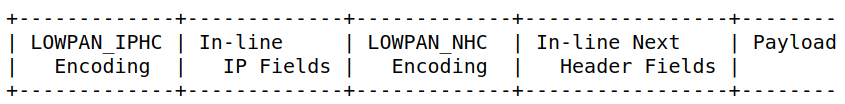
\includegraphics[width=1.0\textwidth]{img/6lowpan-header.png} % first figure itself
        \caption{\label{fig:6lowpan-header} IPv6 Next Header Compression}
    \end{minipage}\hfill
    \begin{minipage}{0.5\textwidth}
        \centering
        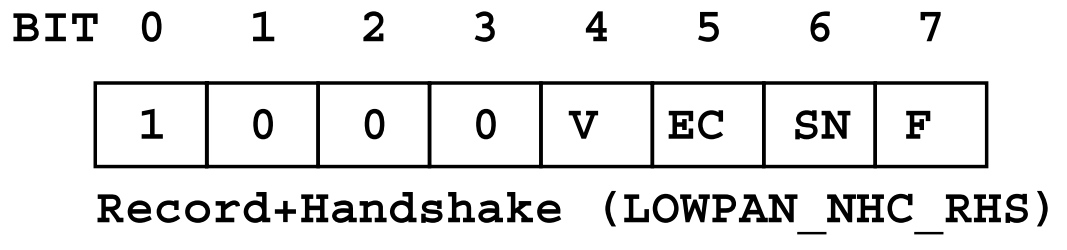
\includegraphics[width=1.0\textwidth]{img/6lowpan-ghc-rhs.png} % second figure itself
        \caption{\label{fig:6lowpan-ghc-rhs} LOWPAN\_NHC\_RHS structure}
    \end{minipage}
\end{figure}


All of the cases follow the same basic idea, for this reason I'll only exemplify
one of them. Each \gls{dtls} fragment is carried over in the UDP payload. In this case,
the UDP payload carries a header-like payload (the DTLS record header).
Figure \ref{fig:6lowpan-header} shows the way IPv6 next header compression is done.
The authors use the same value for the \codeword{LOWPAN_NHC Encoding} field (defined in \cite{RFC6282})
as in \codeword{RFC7400} and define the format of the \codeword{In-line Next Header Fields}
(defined in \cite{RFC6282}), which is the compressed DTLS content. The \codeword{LOWPAN_IPHC Encoding}
and \codeword{In-Line IP Fields} fields are used in the IPv6 header compression
and are not in the scope of the paper.

I will exemplify the case where both, the record and the Handshake headers are compressed.
In this case \codeword{LOWPAN_NHC Encoding} will contain the \codeword{LOWPAN_NHC_RHS}
structure (depicted in figure \ref{fig:6lowpan-ghc-rhs}), which is the compressed form of the Record and Handshake headers. The
parts that are not compressed will be contained in the \codeword{Payload} part.
The first four bits represent the ID field and in this case they're fixed to \codeword{1000},
so that the decompressor knows what is being compressed (\textit{i.e} how to interpret
the structure that follows the ID bits). If the \codeword{F} field of the \codeword{LOWPAN_NHC_RHS} structure contains the
bit \codeword{0}, it means that the handshake message is not fragmented, so
the \codeword{fragment_offset} and \codeword{fragment_length} fields are
elided from the Handshake header (common case when a handshake message is not bigger than
the maximum header size), meaning that they're not going to be sent at
all (\textit{i.e.} they're not going to be present in the \codeword{Payload} part).
If the \codeword{F} bit has the value \codeword{1}, the \codeword{fragment_offset}
and \codeword{fragment_length} fields are carried inline (\textit{i.e.} they're
present in the \codeword{Payload} part). The remaining two fields define similar
behavior for other header fields (some of them assume that some default value is present, when a field is elided).
The \codeword{length} field in the Record and Handshake headers are always elided,
since they can be inferred from the lower layers.

The evaluation showed that the compression can save a significant number of bits:
the Record header, that is included in all messages can be compressed by \codeword{64 bits}
(\textit{i.e.} by \codeword{62\%}).

There is also a proposal for TCP header compression for 6LoWPAN\cite{I-D.draft-aayadi-6lowpan-tcphc-01},
which if adopted, in many cases can compress the mandatory \codeword{20 bytes} TCP header
into \codeword{6 bytes}. This means that the same ideas can be applied to TCP and
TLS as well.

Later, in 2013, Raza \textit{et al.} proposed a security scheme called Lithe\cite{LitheLig40:online},
which is a lightweight security solution for \gls{coap} that uses the same DTLS header
compression technique as in \cite{6LoWPANC53:online} with the goal of implementing
it as a security support for \gls{coap}.\gls{coap}\cite{RFC7959} is a specialized
RESTful Internet Application Protocol for constrained devices. It's designed to easily
translate to HTTP, in order to simplify its integration with the web,
while also meeting requirements such as multicast support and low overhead.
\gls{coap} is like "HTTP for constrained devices".
\gls{coap} can run on most devices that support UDP or a UDP-like protocol.
\gls{coap} mandates the use of \gls{dtls} as the underlying security protocol for
authenticated and confidential communication.

The authors evaluated their system in a simulated environment in Contiki OS and
they obtained significant gains in terms of packet size (similiar numbers to the
ones obsever in \cite{6LoWPANC53:online}), energy consumption (in average \codeword{15\%} less
energy is used to transmitting and receive compressed packets), processing time
(the compression and decompression time of DTLS headers is almost negligible)
and network-wide response times(up to \codeword{50\%} smaller RTT). The
gains in the mentioned measures are the largest when the compression avoids
fragmentation (in the paper, for payload size of \codeword{48 bytes}).

Angelo \textit{et al} \cite{Security5:online} proposed to integrate the \gls{dtls} protocol
inside the \gls{coap}, while also exploiting \gls{ecc} optimizations and minimizing
ROM occupancy. They've implemented their solution on an off-the-shelf mote platform
and evaluated its performance. \gls{dtls} was designed to protect web application communication, as a result,
it has a big overhead in \gls{iot} scenarios. Besides that, it runs over UDP,
so additional mechanisms are needed to provide the reliability and ordering
guarantee. With this in mind, the authors wanted to design a version of \gls{dtls}
that's both: minimizes the code size and the number of exchanged messages, resulting
in an optimized Handshake protocol.

In order to minimize the code size occupied by the \gls{dtls} implementation, they
decided to delegate the tasks of \textbf{reliability} and \textbf{fragmentation} to
\gls{coap}. This means that the code responsible for those functionalities,
can be removed altogether from the \gls{dtls} implementation, thus reducing ROM
occupancy. This part of their work was based on an informational RFC draft\cite{I-D.draft-keoh-dtls-profile-iot-00}, in which the
authors profiled \gls{dtls} for \gls{coap}-based \gls{iot} applications and proposed
the use of a RESTful \gls{dtls} Handshake which relies on \gls{coap} block-wise
transfer to address the fragmentation issue.

To achieve this they  proposed the use of a RESTful \gls{dtls} connection as a \gls{coap} resource,
which is created when a new secure session is requested.
The authors exploit the the \gls{coap}s capability to provide connection-oriented
communication offered by its message layer. In particular, each \codeword{Confirmable}
\gls{coap} message requires an \codeword{Acknowledgement} message\cite{RFC7252T66:online},
which acknowledges that a specific \codeword{Confirmable} message has arrived, thus
providing reliable retransmission.

Instead of leaving the fragmentation function to \gls{dtls}, it was
delegated to the block-wise transfer feature of \gls{coap}\cite{RFC7959}, which was developed
to support transmission of large payloads. This approach has two advantages: first, the code in the \gls{dtls}
layer responsible for this function can be removed, thus reducing ROM occupancy
and second, the fragmentation/reassembly process burdens the lower Layers
with state that is better managed in the application layer.

The authors also optimized the implementation of basic operations on which
many security protocols, such as \gls{ecdh} and \gls{ecdsa} rely upon. The first
optimization had to do with modular arithmetic on large integers. A set of optimized
assembly routines based on \cite{Comparin25:Online} allow the improved use of
registers, reducing the number of memory operations needed to perform
operations such as multiplications and square roots on devices with \codeword{8-bit}
registers.

Scalar multiplication is often the most expensive operation in \gls{ec} based
cryptography, therefore optimizing it is of high interest. The authors used a
technique called \textit{IBPV} described in \cite{LowcostS87:online}, which is based on precumputation
of a set of Discrete Log pairs. I will refrain from going into the mathematical details,
since they're not relevant for this description. The \textit{IBPV} technique was used
to improve the performance of the \gls{ecdsa} signature and was also extended to the
\gls{ecdh} protocol. In order to reduce the time it takes to do the \gls{ecdsa}
signature verification, the \textit{Shamir trick} was used, which allows
to perform the sum of two scalar multiplications (frequent operation in \gls{ec} cryptography)
faster than performing two independent scalar multiplications.

The results showed that the \gls{ecc} optimizations
outperform the scalar multiplication in the state of the art class 1 device platforms,
while also improving the the network lifetime by a factor of up to $6.5$ with
respect to a standard, non-optimized implementation. Leaving reliability and
fragmentation tasks to \gls{coap}, reduces the \gls{dtls} implementation code size
by approximately $23\%$.

%\end{enumerate}

\section{Background}
%
\todo{Tell that first I describe the parts of TLS that are common to both and then
specialize for TLS 1.2 and TLS 1.3}
%
\section{The TLS Protocol}
TLS stands for Transport Layer Security, it's a \textbf{client-server} protocol
that runs on top a \textbf{connection-oriented and reliable transport protocol},
such as \textbf{TCP}. Its main goal is to provide \textbf{privacy} and \textbf{integrity}
between the two communicating peers. Privacy implies that a third party will not
be able to read the data, while integrity means that a third party will not be
able to alter the data.

In the TCP/IP Protocol Stack, \gls{tls} is placed between the \textbf{Transport}
and \textbf{Application} layers. It's designed to make the application developer's
life easier: all the developer has to do is create a "secure" connection, instead
of a "normal" one.

\todo{Re-write what's below. It's good to include something like this,
but I need to work on the wording.}
From the top-level view, in a typical connection, there are three basic steps
that \gls{tls} is responsible for:
\begin{enumerate}
  \item \textbf{Negotiate security parameters} - the communicating peers agree on
  a set of security parameters to be used in a \gls{tls} connection, such as the
  algorithm used for bulk data encrytion, as well as the secret keys.
  \item \textbf{Authenticate one to another} - usually only the server authenticates
  to the client.
  \item \textbf{Communicate securely} - use the negotiated security parameters
  to encrypt and authenticate the data, communicating securely one with another.
\end{enumerate}


%%% NOTE: place this in intro? Is this even needed?
%%% NOTE: review, rephrase
%%% NOTE: find better placement
\subsubsection{SSL vs TLS: What's The Difference?}
You will find the names \gls{ssl} and \gls{tls} used interchangeably in the literature,
so I think it's important to distinguish both. \gls{tls} is an evolution of the \gls{ssl} protocol. The protocol changed
its name from \gls{ssl} to \gls{tls} when it was
standardized by the \gls{ietf}.\gls{ssl}
was a proprietary protocol owned by Netscape Communications, and The \gls{ietf}
decided that it was a good idea to standarize it, which resulted in \codeword{RFC 2246} \cite{RFC2246},
specifying \gls{tls} 1.0, which was nothing more than a new version \gls{ssl} 3.0,
very few changes were made.
%
% TODO: add some data supporting the TLS 1.2 usage claim
In this document, I'll be concentrating on \gls{tls} 1.2 and \gls{tls} 1.3 protocols.
The first one is the most recently standardized version of \gls{tls} and the latter
is currently and in-draft version with many improvements and optimizations relevant
for the topic of this dissertation. Despite the protocol name not suggesting it \gls{tls} 1.3 is
very different from \gls{tls} 1.2, in fact, it should've probably been called
\gls{tls} 2.0 instead. For this reason, I will first describe what is common to
both protocols and then go into the relevant details about each one.
%

\todo{Explain what RFCs are?}
%
\subsection{Security Services}
%
\gls{tls} provides the following 3 security services:
\begin{itemize}
\item \textbf{authentication} - both, \textbf{peer entity} and \textbf{data origin} (or \textbf{integrity})
authentication.
\subitem \textbf{peer entity authentication} - we can be sure that we’re talking to certain entity, for example, \codeword{www.google.com}.
This is achieved thought the use of \textbf{asymmetrical} or \gls{pkc} (for example, \codeword{RSA} and \codeword{DSA})
or \textbf{symmetric key cryptography}, using a \gls{psk}.
\item \textbf{confidentiality} - the data transmitted between the communicating
entities (the client and the server) is encrypted. Symmetric cryptography is
used of data encryption (for exmaple, \codeword{AES}).
\item \textbf{integrity} (also called \textbf{data origin authentication}) - we can be sure that the data was not modified or forged,
\textit{i.e.}, be sure that the data that we’re receiving is coming from the expected entity (for example, we can be sure
that the \codeword{index.html} file sent to us when we connected to \codeword{www.google.com} in fact
came from \codeword{www.google.com} and that it was not modified (i.e tampered with) en
route by an attacker (\textbf{data integrity}). This is achieved through the use
of a keyed \gls{mac} or an \gls{aead} cipher.
\end{itemize}

Despite using \gls{pkc}, \gls{tls} does \textbf{not} provide \textbf{non-repudiation services}:
neither \textbf{non-repudiation with proof of origin}, which addresses the user denying
having sent a message, not \textbf{non-repudiation with proof of delivery}, which
addresses the user denying the receipt of a message. This is due to the fact, that
instead of using \textbf{digital signatures}, either a keyed \gls{mac} or an \gls{aead}
cipher is used, both of which require a \textbf{shared secret} to be used.

You are not required to use all of the 3 security services in every situation.
You can think of \gls{tls} as a framework that allows you to select which security
services you want to use for a communication session. As an example, you might
ignore certificate validation, which means you're ignoring the \textbf{authentication}
guarantee. There are some differences regarding this claim between \gls{tls} 1.2
and \gls{tls} 1.3, for example, while in the first you have a \codeword{null}
cipher (no authentication, no confidentiality, no integrity), in the latter
this is not true, since it deprecated all non-\gls{aead} ciphers in favor of
\gls{aead} ones.

\subsubsection{Cipher Spec vs Cipher Suite}

The meaning of these terms differs in \gls{tls} 1.2 and \gls{tls} 1.3. For \gls{tls} 1.2,
\textbf{cipher spec} defines the message encryption algorithm and the message
authentication algorithm, while the \textbf{cipher suite} is the \textbf{cipher spec},
alongside the definition of the \textbf{key exchange} algorithm and the \gls{prf} (used in key generation). In \gls{tls} 1.3, the
 \textbf{cipher spec} has been removed altogether, since the  \textbf{ChangeCipherSpec}
 protocol has been removed. The concept of \textbf{cipher suite} has been updated
 to define the pair of \gls{aead} algorithm and hash function to be used with
 \gls{hkdf}: in \gls{tls} 1.3 the  \textbf{key exchange} algorithm is negotiated via
 extensions. You'll find more details on this below.

\subsection{TLS (Sub)Protocols}

In reality \gls{tls} is composed of several protocols(illustrated in \ref{fig:tls-subprotocols}), a brief description of each
one of which follows:
\begin{itemize}
  \item \textbf{\gls{tls} Record Protocol} - the lowest layer in \gls{tls}. It's
  the layer that runs directly on top of \textbf{TCP/IP} and it serves as an
   \textbf{encapsulation for the remaining sub-protocols} (\codeword{4} in case of \gls{tls} 1.2
   and \codeword{3} in case of \gls{tls} 1.3). To the  \textbf{Record Protocol},
   the remaining sub-protocols are what \codeword{TCP/IP} is to \codeword{HTTP}.
   A \gls{tls} Record is comprised of 4 fields, with the first 3 comprising the
   \gls{tls} Record header: a 1-byte record \codeword{type},
   specifying the type of record that's encapsulated (ex: value \codeword{0x16}
   for the handshake protocol), a 2-byte \codeword{TLS version} field, a
   2-byte \codeword{length} field (which means that a maximum \gls{tls} Record size
   is of \codeword{16384} bytes), specifying the length of the data in the record, excluding
   the header itself and a \codeword{fragment} field whose size in bytes is specified
   by the \codeword{length} field, which contains data that's
   transparent to the Record layer and should be dealt by a higher-level protocol,
   specified by the \codeword{type} field. This is illustrated in figure \ref{figure:tls-record-header}.
  \item \textbf{\gls{tls} Handshake Protocol} - the core protocol of \gls{tls}.
  Allows the communicating peers to \textbf{authenticate} one to another and negotiate
  a \textbf{cipher suite} (\textbf{cipher suite} and key exchange algorithm in case of \gls{tls} 1.3) which will be used to provide the security services. For \gls{tls} 1.2,
  \textbf{compression} method is also negotiated here.
  \item \textbf{\gls{tls} Alert Protocol} - allows the communicating peers to
  signal potential problems.
  \item \textbf{\gls{tls} Application Data Protocol} - used to transmit data securely.
  \item \textbf{\gls{tls} Change Cipher Spec Protocol} (removed in \gls{tls} 1.3) -
  used to activate the initial \textbf{cipher spec} or change it during the connection.
\end{itemize}

% src: https://tex.stackexchange.com/questions/5769/two-figures-side-by-side
\begin{figure}
    \centering
    \begin{minipage}{0.5\textwidth}
        \centering
        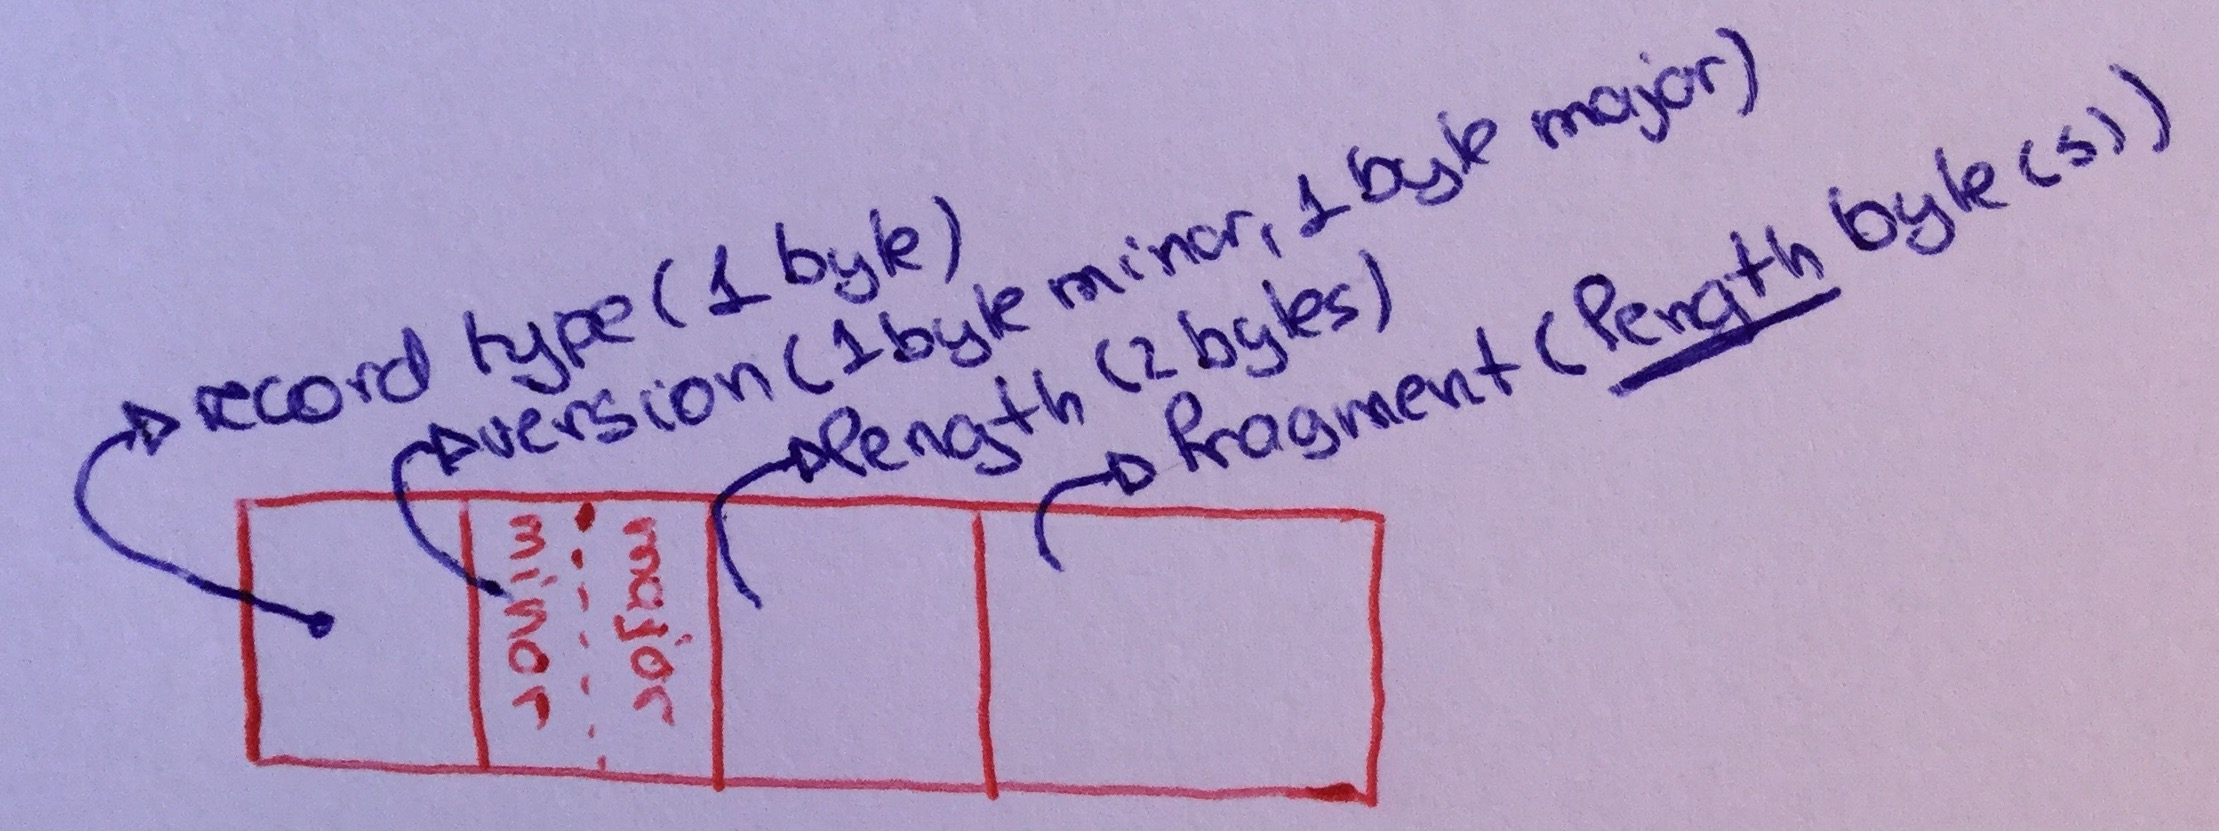
\includegraphics[width=1.0\textwidth]{img/record-header.jpg} % first figure itself
        \caption{\label{fig:tls-record-header} TLS Record header}
    \end{minipage}\hfill
    \begin{minipage}{0.5\textwidth}
        \centering
        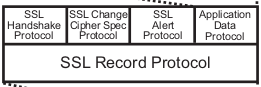
\includegraphics[width=1.0\textwidth]{img/tls-sub-protocols.png} % second figure itself
        \caption{\label{fig:tls-subprotocols} TLS (Sub)protocols and Layers}
    \end{minipage}
\end{figure}

\paragraph{TLS Connections and Sessions}

\todo{define what it means to be cryptographically protected?}

It's important to distinguish between a \textbf{TLS session} and a \textbf{TLS connection}.
\begin{itemize}
  \item \textbf{TLS sesion} - assosciation between two communicationg peers that's
  created by the \textbf{TLS Handshake Protocol}, wich defines a set of negotiated paramters
  (cyrptographic and others, depending on the \gls{tls} version, such as
  the compression algorithm) that are used by the \textbf{TLS connections associated
  with that session}. A single \textbf{TLS session} can be shared among multiple
  \textbf{TLS connections} and its main purpuse is to avoid the expensive negotiation
  of new parameters for each \textbf{TLS connection}. For example, let's say
  you download an \gls{html} page over \gls{https} and that page referrences
  some images from that same server, also using \gls{https}, instead of your
  web browser negotiating a new \gls{tls} session again, it can re-use the the
  one you established to download the \gls{html} page in the first place,
  saving time and computational resources. Session resumption can be done using various
  approaches, such as \textbf{session identifiers}, described throughout \codeword{Section 7.4}
  of \codeword{RFC 5246} \cite{RFC5246}, \textbf{session tickets}, defined in
  \codeword{RFC 5077} \cite{RFC5077}. \todo{Re-write example better.}
  \item \textbf{TLS connection} - used to actually transmit the cryptographically
  protected data. For the data to be cryptographically protected, some parameters,
  such as the \codeword{secret keys} used to encrypt and authenticate the transmitted
  data need to be established; this is done when a \textbf{TLS session} is created,
  during the \textbf{TLS Handshake Protocol}.
\end{itemize}

\subsubsection{\gls{tls} Record Processing}
A \gls{tls} record must go through some processing before it can tbe sent over the netwrok.
This processing involves the following steps (\codeword{4} for \gls{tls} 1.2 and \codeword{3} for \gls{tls} 1.3):

\begin{enumerate}
  \item \textbf{Fragmentation} - the \gls{tls} \codeword{Record Layer} takes arbitrary-length data and \textbf{fragments}
  it into manageable pieces: each one of the resulting fragments is called a \codeword{TLS Plaintext}.
  Client message boundaries are not preserved, which means that multiple messages
  of the same type may be placed into the same fragment or a single message may
  be fragmented across several records.
  \item  \textbf{Compression} (removed in \gls{tls} 1.3) - the \codeword{TLS Record Layer} compresses the
  \codeword{TLSPlaintext} structure according to the negotiated compression method,
  outputting \codeword{TLSCompressed}. Compression is optional. If the negotiated compression
  method is \codeword{null}, \codeword{TLSCompressed} is the same as \codeword{TLSPlaintext}.
  \item \textbf{Cryptographic Protection} - in case of \gls{tls} 1.2, either an
  \gls{aead} cipher or a separate encryption and \gls{mac} functions transform a
  \codeword{TLSCompressed} fragment into a \codeword{TLSCipherText} fragment. In case
  of \gls{tls} 1.3, the \codeword{TLSPlaintext} fragment is transformed into a \codeword{TLSCipherText}
  by applying an \gls{aead} cipher.
  \item Append the \textbf{TLS Record Header} - encapsulate \codeword{TLSCipherText}
  in a \codeword{TLS Record}.
\end{enumerate}

\begin{wrapfigure}{r}{0.4\textwidth}
\centering
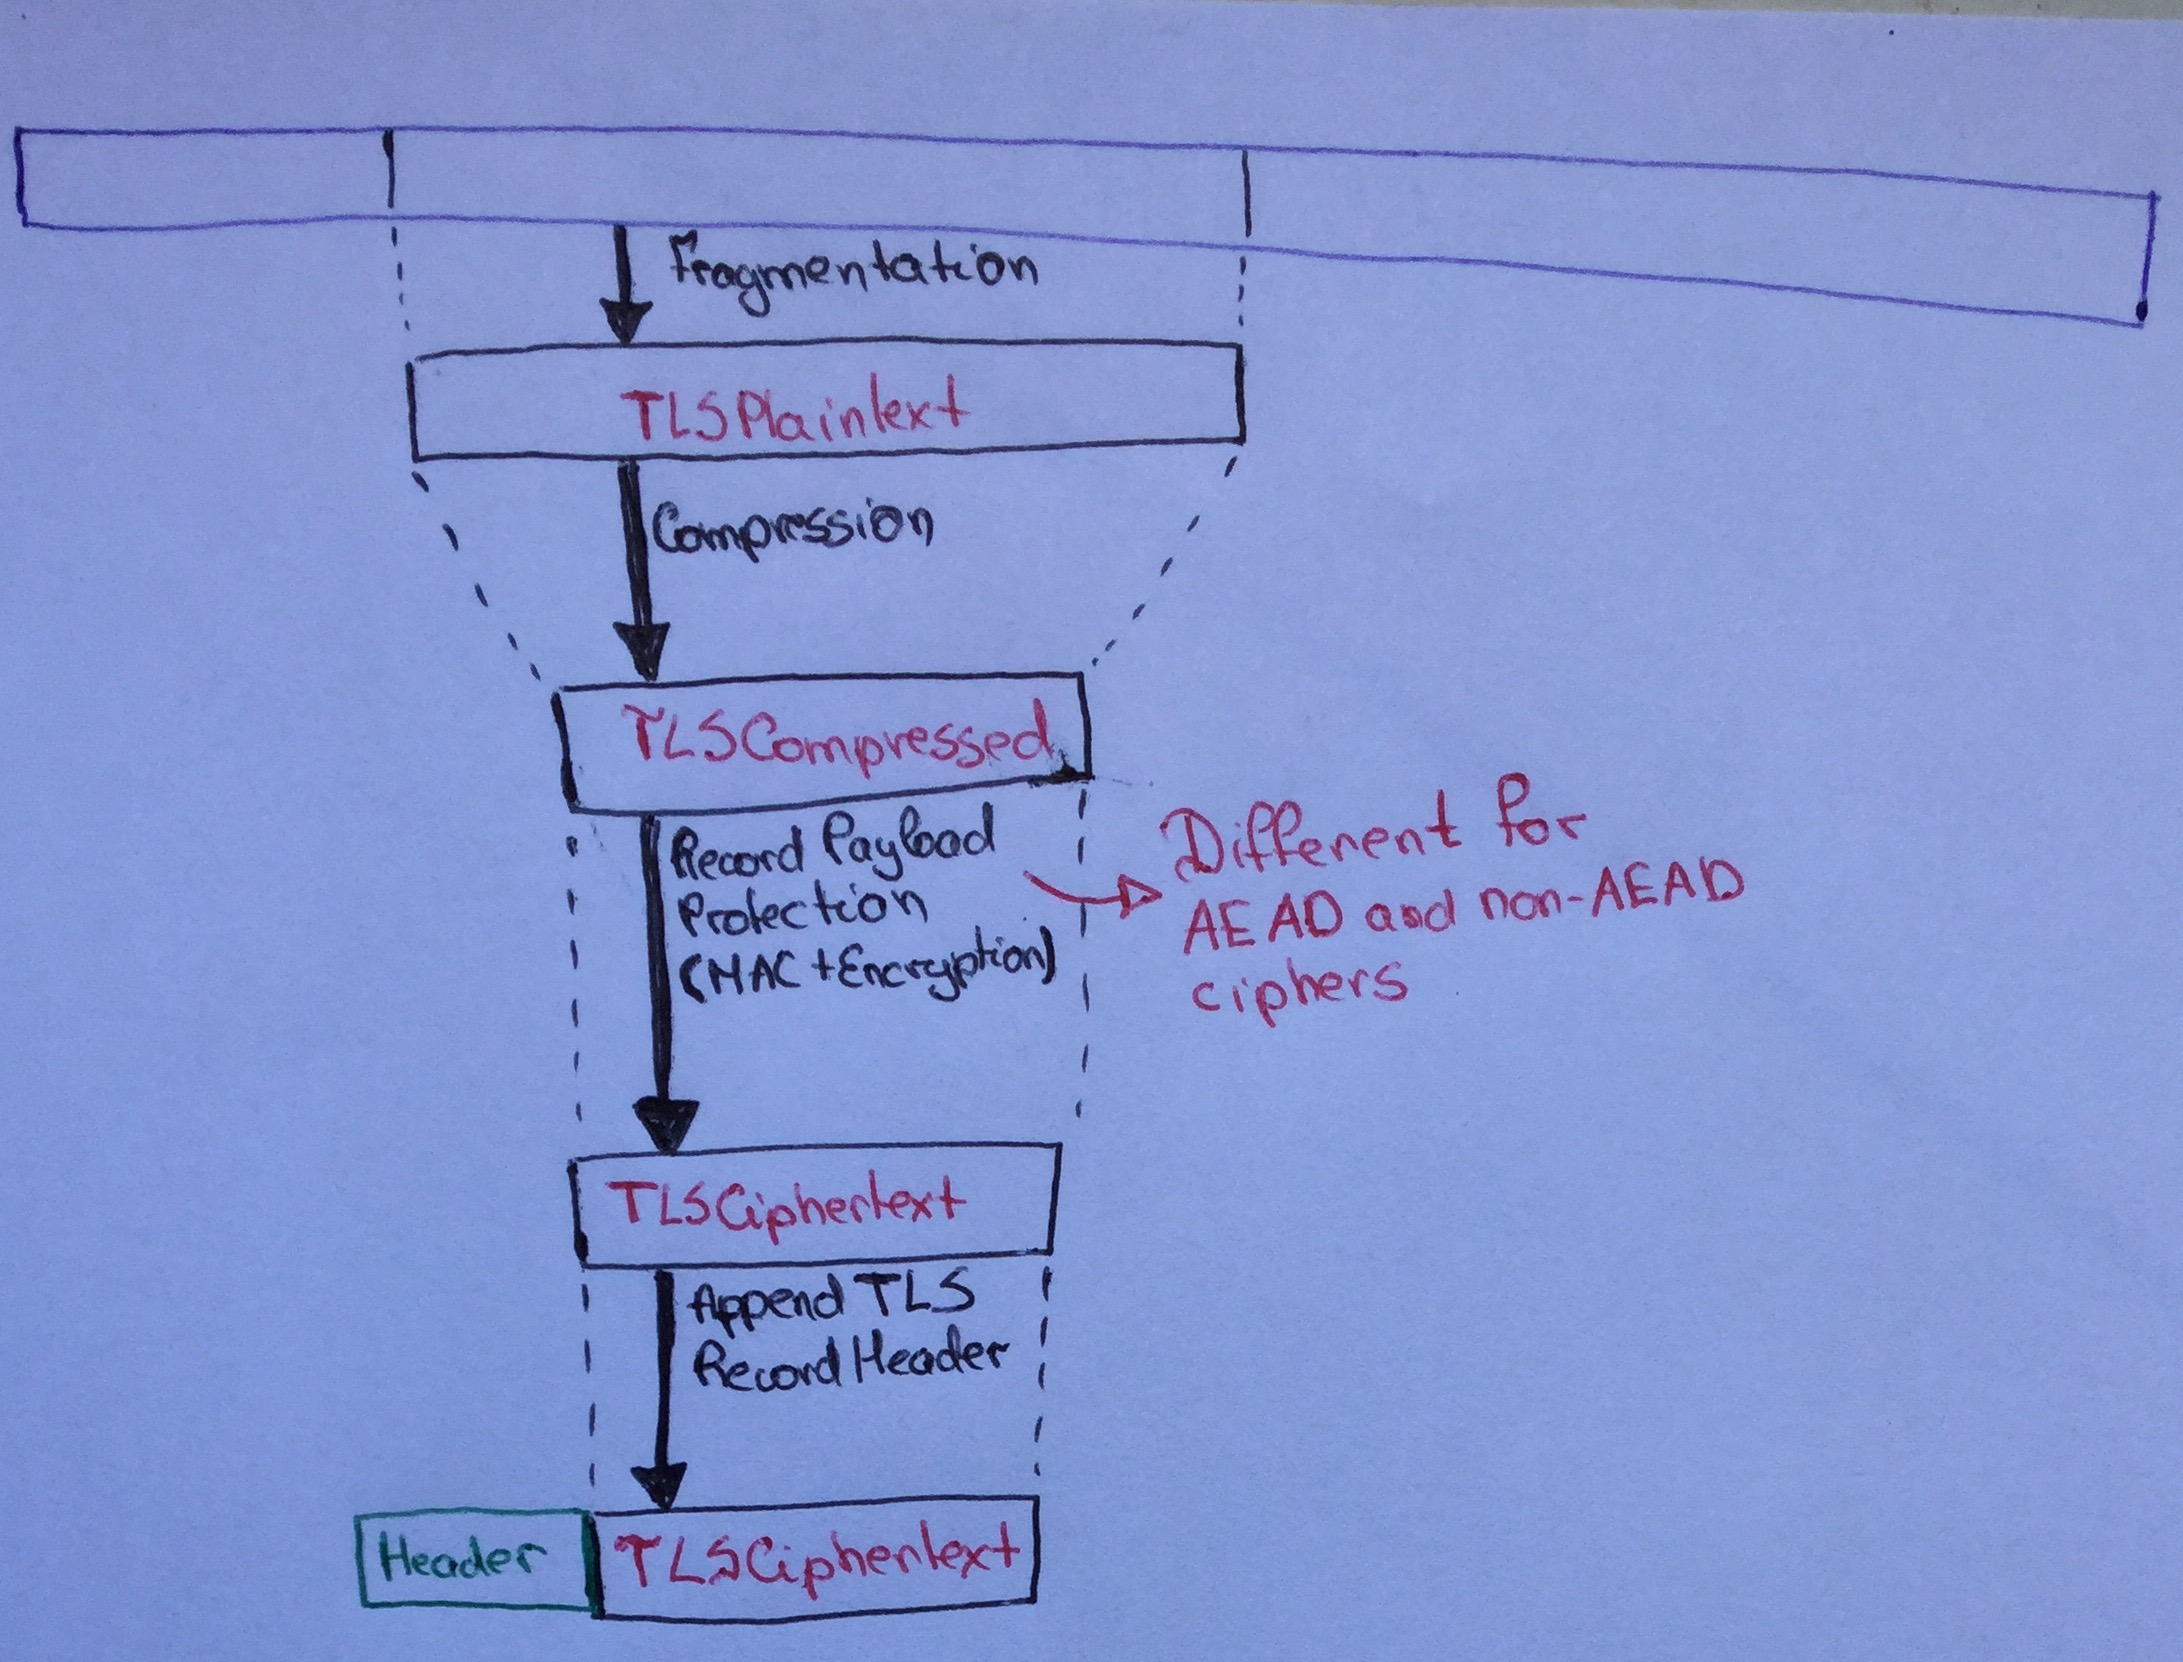
\includegraphics[width=0.7\textwidth]{img/tls-record-processing.jpg}
\caption{\label{fig:tls-record-processing}TLS Record Processing}
\end{wrapfigure}

The process described above, as well as the structure names are depicted in figure \ref{fig:tls-record-processing}.
Step \codeword{2} is not present in \gls{tls} 1.3. The structure names are exactly as the appear in the \gls{tls} specifications.

\subsection{TLS Keying Material}
Secret keys are at the base of most cryptographic operations.
In order for both communicating peers to be able to encrypt and decrypt data
using symmetric cyrpto aglorithms, they need to \textbf{share} the same key
somehow. In \gls{tls}, both, the client and a server derive the \textbf{same set of keys}
independetely, through the exchanged messages in the \gls{tls} Handshake Protocol.

When communicating with one anohter, the client uses one key to
encrypt the data to be sent to the server and another different key to decrypt the data
that it receives from the server. This means that in order to deal with data
encryption and decryption, both of the communicating entities have two keys:
one to encrypt the outgoing data and one to decrypt the incoming data. Those keys
have different names in \gls{tls} 1.2 and \gls{tls} 1.3, but they serve the same
basic purpose. In this general description, I'll refer to them as \codeword{client_write key}
(used by the client to encrypt the data to be sent), \codeword{client_read_key}(used by the client to
decrypt the incoming data from the server), \codeword{server_write_key}(used by the server to encrypt
the data to be sent) and \codeword{server_read_key}(used by the server to decrypt the incoming
data from the client). Note, that the following relationships must hold:
\codeword{client_write_key == server_write_key} and \codeword{client_read_key == server_write_key}.

Besides the secret keys mentioned previously, in \gls{tls} 1.2 you might also have other ones,
depending on the cipher suite in use. \todo{Describe this in a little more detail,
giving examples, when describing TLS 1.2 Key Managment}.

\gls{tls} 1.3's keying material generation is a little more complex, since different
keys are used to encrypt data throughout the Handshake Protocol, as well a new key
is generated for the Application Data protocol. This can be explained by the fact
that while in \gls{tls} 1.2 the data only begins to be encrypted after the handshake
is complete, in the Application Data protocol, the encryption begins earlier,
\gls{tls} 1.3, with some of the Hanshake messages encrypted, as well as features
such as \textbf{early client/server data} and \textbf{0-RTT Data}.

With this the common description of the \gls{tls} of protocols ends and we'll jump
into the specifics of the two verions. I'll be mostly concentrating on the
 \textbf{Handshake Protocol}, since this is where my work will be concentrated and
 it's the main part, where the most interesting and important things happen.

\subsection{TLS 1.2}
The latest standardized version of \gls{tls} is 1.2 and it's defined in \codeword{RFC 5246} \cite{RFC5246}.
\todo{DESCRIBE TLS 1.2 in genreal, put images of handshakes here, later refer to them
in the specific parts, just like the tls RFCs do}.

\section{TLS 1.2 Keying Material Generation}
The generation of secret keys, used for various cryptographic operations involves the
following steps (in order):

\begin{itemize}
  \item Generate the \textbf{premaster secret}
  \item From the \textbf{premaster secret} generate the \textbf{master secret}
  \item From the \textbf{master secret} generate the various secret keys, which
  will be used in the cryptographic operations.
\end{itemize}

\todo{talk about all of the keys present in TLS 1.2 HERE}

\section{TLS 1.2 Key Exchange Methods}
The way the \textbf{permaster secret} is generated depends on the key exchange
method used. In fact, this is the only phase of the keying material generation
phase that is variable for a fixed cipher suite (because a cipher suite defines
the \gls{prf} function to be used), the rest remains exactly the same. The derivation
of the \textbf{master secret} from the \textbf{premaster secret}, as well as the
derivation of the bulk encryption keys, \gls{mac} keys and \gls{iv}s from the \textbf{master secret}
that follows \textbf{is not impacted by the key exchange method} in use.

You have quite a few choices when it comes to key exchange methods. Some of them
are defined in the base spec (\codeword{RFC5246} \cite{RFC5246}), while others
in separate \codeword{RFCs} (such as the \gls{ecc} based key exchange, specified
in \codeword{RFC4492} \cite{RFC4492}).

The base spec specifies 4 key exchange methods, one using \gls{rsa} and 3 using
\gls{dh}:

\begin{itemize}
  \item static \gls{rsa} (\codeword{RSA}) [removed in \gls{tls} 1.3] - the client generates the \gls{pms}, encrypts it with the
  server's \gls{pubk} (which it obtained from the server's \codeword{X.509}certificate),
  sending it to the server, which decrypts it using the corresponding \gls{privk}.
  This key exchange method offers authenticity, but does not offer \gls{pfs}.
  \item anonymous \gls{dh} (\codeword{DH_annon}) [removed in \gls{tls} 1.3] - a \gls{dh} key exchange is
  performed and an \textbf{ephemeral} key is generated, but the exchanged \gls{dh}
  parameters are \textbf{not authenticated}, making the resulting key exchange
  vulnerable to \gls{mitm} attacks. \gls{tls} 1.2 spec states that cipher suites
  using \codeword{DH_annon} \textbf{must not} be used, unless the application
  layer explicitly requests so. This key exchange offers \gls{pfs}, but no
  authenticity.
  \item fixed/static \gls{dh} (\codeword{DH}) [removed in \gls{tls} 1.3] - the server's/client's public \gls{dh} parameter
  is embedded in its certificate. This key exchange method offers authenticity,
  but does not offer \gls{pfs}.
  \item epehemeral \gls{dh} (\codeword{DHE}) - each run of the protocol, uses
  different pubic \gls{dh} parameters, which are generated dynamically. This results
  in a different, epehemeral key being generated every time. The public parameters
  are then digitally signed in some way, usually using the sender's private
  \gls{rsa} (\codeword(DHE_RSA)) or \gls{dsa} (\codeword{DHE_DSS}) key. This key
  exchange offers both authenticity and \gls{pfs}.
\end{itemize}

When either of the \gls{dh} variants is used, the value resulting from the exchange is used
as the \gls{pms} (without the leading \codeword{0}'s). Usually, only the server's
authenticity is desired, but client's can also be achieved if it provides the
server its certificate. Whenever the server is authenticated, the server is secure
against \gls{mitm} attacks. Table \ref{kemps} summarizes the security properties
offered by each key exchange method.

\begin{table}[]
\centering
\caption{Key exchange methods and security properties}
\label{kemsp}
\begin{tabular}{|l|c|l|}
\hline
\textbf{Key Exch Meth} & \multicolumn{1}{l|}{Authentication} & PFS                    \\ \hline
RSA                          & X                                   &                        \\ \hline
DH\_anon                     & \multicolumn{1}{l|}{}               & \multicolumn{1}{c|}{X} \\ \hline
DH                           & X                                   &                        \\ \hline
DHE                          & X                                   & \multicolumn{1}{c|}{X} \\ \hline
\end{tabular}
\end{table}

Note that in \gls{tls} 1.3, all of static \gls{rsa} and \gls{dh} cipher suites
have been removed: all of the \gls{pubk} exchange methods now provide \gls{pfs}.
Even though, anonymous \gls{dh} has also been removed from \gls{tls} 1.3, you can
still have unauthenticated connections by either using \textbf{raw public keys} \cite{RFC7250}
or by not verifying the certificate chain and any of it's contents.

\todo{NOTE: I did't cover specifics of how the client generates the premaster secret, etc}

The \gls{ecc}-based key exchange (\gls{ecdh} and \gls{ecdhe}) and authentication (\gls{ecdsa})
algorithms are defined in \codeword{RFC4292} \cite{RFC4292}, which is also referenced
in \codeword{RFC5246} \cite{RFC4256}. The document introduces five new
\gls{ecc}-based key exchange algorithms, all of which use \gls{ecc} to compute
the \textbf{premaster secret}, differing only in whether the negotiated
keys are epehemeral (\gls{ecdh}) or long-term (\gls{ecdhe}), as well as the mechanism (if any) used to
authenticate them. Three new \gls{ecdsa} \textbf{client authentication} mechanisms are also defined,
differing in the algorithms that the certificate must be signed with, as well
as the key exchange algorithms that they can be used with.
Those features are negotiated through the \gls{tls} Extension Mechanism.

\subsection{TLS 1.2 Handshake Protocol}


\begin{figure}
\centering
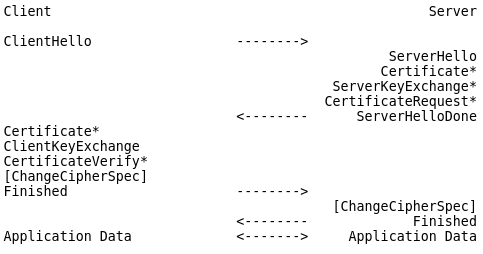
\includegraphics[width=0.9\textwidth]{img/tls-12-full-handshake.png}
\caption{\label{fig:tls-12-handshake} TLS 1.2 message flow for a full handshake}
\end{figure}


In this phase the client and the server agree on which version of the \gls{tls}
protocol to use, authenticate one to another and negotiate items like
the cipher suites and the compression method to use. Figure \ref{fig:tls-12-handshake} shows the message flow for the
full \gls{tls} 1.2 handshake. Note that \codeword{*} indicates situation-dependent
messages that are not always sent, while \codeword{ChangeCiperSpec} is a separate
protocol, rather than a message type.

As I explained before every \gls{tls} Handshake message is encapsulated within
a \gls{tls} Record. The actual Handshake message is contained within the
\codeword{fragment} of the \gls{tls} Record. The Record type for a Handshake
message is \codeword{0x16}. The Handshake message has the following structure:
a 1-byte \codeword{msg_type} field (specifies the Handshake message type),
a 2-byte \codeword{length} field (specifies the length of the \codeword{body})
and a \codeword{body} field, which contains a structure depending on the
\codeword{msh_type} (similar to \codeword{fragment} field in a \gls{tls} Record).

Now, I will describe a typical handshake message flow. I will only be mentioning
the most important field of each message.

\todo{I don't have space to put all of the structures and things sent in every
handshake message type (ex: ClientHello.session\_id)}

The connections begins with the client sending a \codeword{ClientHello}, containing
.\codeword{random}, \codeword{cipher_suites} and \codeword{compresison_methods},
among other fields. A 32-byte \codeword{random}
(3-bytes gmt unix time + 27 cryptographically random bytes) value that are used
as an input to the \gls{prf} when generating the \textbf{master secret}, which
will cause to
contains a \textbf{list} of cipher suites (\codeword{cipher_suites}) and
compression methods (\codeword{compression_methods}) that the client supports, ordered by
preference, with the most preferred one appearing first.

\subsection{Do We Really Need Two Randoms: One From Client and One From Server?}
\todo{YES, replay attacks.}

\todo{Mention HelloRequest}
%
\paragraph{Notes and Comments.}
This is an example of a paragraph. Note the styling.

\subsection{TLS 1.3}
Despite the protocol name not suggesting it \gls{tls} 1.3 is
very different from \gls{tls} 1.2, in fact, it should've probably been called
\gls{tls} 2.0 instead.

\subsubsection{How Do Peers Distinguish Different TLS Versions?}

\todo{Talk about version numbers}

\subsection{TLS Extension Mechanism}

\todo{Describe the Extended ClientHello/ServerHello. Use one description for both,
 TLS 1.2 and TLS 1.3}

\subsection{The Problem With Compression In TLS}

\todo{explain why compression was removed (BEAST and CRIME attacks) and how it
can be fixed.}

\subsection{Theory}

\todo{Explain: public key crypto, certificates, AEAD ciphers}

%
% ---- Bibliography ----
%
\nocite{*}
\bibliographystyle{splncs03}
\bibliography{tls_for_iot,papers}
%
\printglossary[style=long]
%
\end{document}
